\chapter{Técnicas de laboratorio I: seguridad, medida y separación}\label{ch:b1:lab-techniques-1}

Dos estudiantes recristalizan el mismo lote de aspirina y miden su punto
de fusión en el mismo banco calefactor. Uno lee \qty{134}{\celsius}, y el
otro, \qty{136}{\celsius}. ¿Discrepan? ¿Es puro el producto? Ninguna de
las dos preguntas puede responderse solo con los dos números: una medida
solo vale algo con su incertidumbre, y una comparación, solo con una
regla. Este último capítulo reúne la parte práctica del año: cómo leer
los \omterm{def:b1:lab-techniques-1:hazard}{peligros} de lo que hay sobre la mesa, cómo expresar un valor medido
con su incertidumbre y compararlo con otro, y cómo las operaciones
clásicas del laboratorio orgánico --- extracción, filtración,
\omterm{def:b1:lab-techniques-1:recrystallisation}{recristalización}, destilación --- separan un producto de lo que lo rodea,
y cómo se comprueba después que es puro.

\begin{recall}
La \omterm{def:b1:precipitation:solubility}{solubilidad} y la miscibilidad a partir de las fuerzas
intermoleculares, los \omterm{def:b1:intermolecular-forces-solvents:solvent-classes}{disolventes polares} y apolares
(\cref{ch:b1:intermolecular-forces-solvents}); las buretas, las pipetas y
el \omterm{def:b1:titration-methods:titration}{punto final} de una \omterm{def:b1:titration-methods:titration}{valoración} (\cref{ch:b1:titration-methods}). El
volumen escolar (año 10) presentó la extracción líquido--líquido, la
\omterm{def:b1:lab-techniques-1:recrystallisation}{recristalización}, la cromatografía en capa fina y el \omterm{def:b1:extent-q-and-k:fractional-extent}{rendimiento} de una
síntesis; aquí se les ponen números.
\end{recall}

\begin{omfigure}
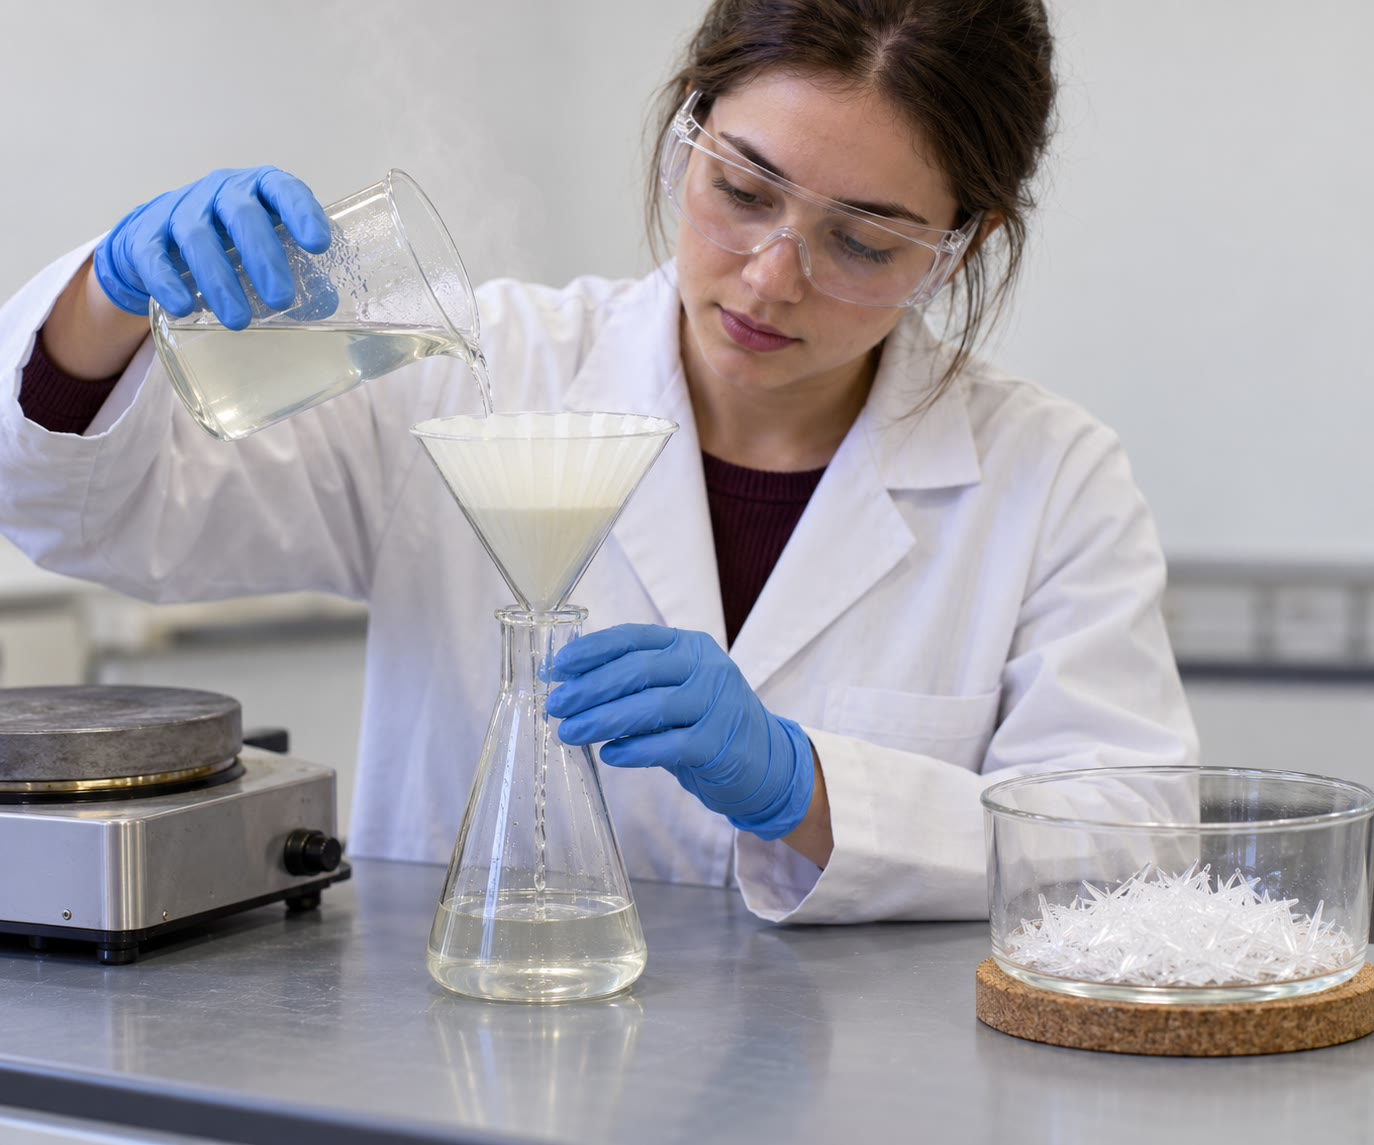
\includegraphics[width=0.5\linewidth]{images/book2/ai/b1-29-recrystallisation.jpg}

{\small Filtración en caliente durante una \omterm{def:b1:lab-techniques-1:recrystallisation}{recristalización}: gafas,
guantes y bata; la disolución caliente pasa a través de un papel de
filtro plegado, que retiene las impurezas insolubles. En la cápsula de la
derecha esperan las agujas de un producto recristalizado.}
\end{omfigure}

\section{Los peligros y sus etiquetas}

\begin{definition}[Peligro y riesgo]\label{def:b1:lab-techniques-1:hazard}
Un \emph{peligro}\index{peligro} es la propiedad intrínseca de una
sustancia (o de una situación) que puede causar daño: la inflamabilidad,
la corrosividad, la toxicidad. El \emph{riesgo}\index{riesgo} es la
probabilidad de que el daño se produzca realmente, y su gravedad, en las
condiciones de uso dadas: depende del peligro y de la exposición
(cantidad, concentración, duración, vía, protección).
\end{definition}

Un \omterm{def:b1:lab-techniques-1:hazard}{peligro} no puede cambiarse sin cambiar la sustancia; un \omterm{def:b1:lab-techniques-1:hazard}{riesgo} se
reduce actuando sobre la exposición: una cantidad menor, una disolución
más diluida, una vitrina de gases, guantes y gafas, o un reactivo menos
peligroso para el mismo trabajo.

\begin{definition}[Etiquetado SGA]\label{def:b1:lab-techniques-1:ghs}
Las etiquetas de los productos químicos siguen el Sistema Globalmente
Armonizado (SGA; en inglés, GHS).
\begin{itemize}
  \item Un \emph{pictograma de peligro}\index{pictograma de peligro} es un
        símbolo negro sobre un rombo blanco de borde rojo; hay nueve, de
        \texttt{GHS01} a \texttt{GHS09}.
  \item La \emph{palabra de advertencia}\index{palabra de advertencia} es
        \emph{Peligro} para las categorías de \omterm{def:b1:lab-techniques-1:hazard}{peligro} más graves y
        \emph{Atención} para las menos graves; una etiqueta lleva solo una,
        la más grave.
  \item Una \emph{indicación de peligro}\index{indicacion de peligro@indicación de peligro} es una frase
        normalizada, codificada con una H seguida de tres cifras, que
        describe un \omterm{def:b1:lab-techniques-1:hazard}{peligro}: H2xx, \omterm{def:b1:lab-techniques-1:hazard}{peligros} físicos; H3xx, \omterm{def:b1:lab-techniques-1:hazard}{peligros} para
        la salud; H4xx, \omterm{def:b1:lab-techniques-1:hazard}{peligros} para el medio ambiente.
  \item Un \emph{consejo de prudencia}\index{consejo de prudencia},
        codificado con una P y tres cifras, indica una medida que debe
        tomarse: P1xx, generales; P2xx, prevención; P3xx, respuesta;
        P4xx, almacenamiento; P5xx, eliminación.
  \item La \emph{ficha de datos de seguridad}\index{ficha de datos de seguridad} es el
        documento que el proveedor entrega con un producto, en secciones
        normalizadas: identificación, \omterm{def:b1:lab-techniques-1:hazard}{peligros}, composición, primeros
        auxilios, lucha contra incendios, manipulación y almacenamiento,
        controles de exposición y protección, propiedades físicas y
        químicas, estabilidad, toxicidad, eliminación y transporte.
\end{itemize}
\end{definition}

\begin{omfigure}
\setlength{\tabcolsep}{5pt}
\begin{tabular}{ccccc}
\begin{tabular}[t]{@{}c@{}}\ghs[1.25cm]{GHS01}\\[2pt]\footnotesize GHS01\\\footnotesize explosivo\end{tabular} &
\begin{tabular}[t]{@{}c@{}}\ghs[1.25cm]{GHS02}\\[2pt]\footnotesize GHS02\\\footnotesize inflamable\end{tabular} &
\begin{tabular}[t]{@{}c@{}}\ghs[1.25cm]{GHS03}\\[2pt]\footnotesize GHS03\\\footnotesize comburente\end{tabular} &
\begin{tabular}[t]{@{}c@{}}\ghs[1.25cm]{GHS04}\\[2pt]\footnotesize GHS04\\\footnotesize gas a presión\end{tabular} &
\begin{tabular}[t]{@{}c@{}}\ghs[1.25cm]{GHS05}\\[2pt]\footnotesize GHS05\\\footnotesize corrosivo\end{tabular} \\[8pt]
\begin{tabular}[t]{@{}c@{}}\ghs[1.25cm]{GHS06}\\[2pt]\footnotesize GHS06\\\footnotesize toxicidad aguda\end{tabular} &
\begin{tabular}[t]{@{}c@{}}\ghs[1.25cm]{GHS07}\\[2pt]\footnotesize GHS07\\\footnotesize nocivo, irritante\end{tabular} &
\begin{tabular}[t]{@{}c@{}}\ghs[1.25cm]{GHS08}\\[2pt]\footnotesize GHS08\\\footnotesize peligro para la salud\end{tabular} &
\begin{tabular}[t]{@{}c@{}}\ghs[1.25cm]{GHS09}\\[2pt]\footnotesize GHS09\\\footnotesize medio ambiente\end{tabular} & \\
\end{tabular}

\smallskip
{\small Los nueve pictogramas del SGA: bomba explotando, llama, llama
sobre un círculo, bombona de gas, corrosión, calavera y tibias cruzadas,
signo de exclamación, peligro para la salud (efectos a largo plazo:
cáncer, mutaciones, reproducción, sensibilización de las vías
respiratorias, aspiración) y medio ambiente.}
% ledger: ghspic:GHS01, ghspic:GHS02, ghspic:GHS03, ghspic:GHS04,
% ghspic:GHS05, ghspic:GHS06, ghspic:GHS07, ghspic:GHS08, ghspic:GHS09
\end{omfigure}

\begin{example}[Leer la etiqueta del etanol]
Una botella de etanol lleva los pictogramas GHS02 y GHS07, la \omterm{def:b1:lab-techniques-1:ghs}{palabra de
advertencia} \emph{Peligro}, y las indicaciones H225 (líquido y vapores
muy inflamables, un \omterm{def:b1:lab-techniques-1:hazard}{peligro} físico cuya categoría exige \emph{Peligro}) y
H319 (provoca irritación ocular grave, un peligro para la salud, que por
sí solo llevaría \emph{Atención}). Entre sus \omterm{def:b1:lab-techniques-1:ghs}{consejos de prudencia}
figuran P210 (mantener alejado del calor, de las chispas y de las llamas
abiertas; no fumar), P233 (mantener el recipiente herméticamente
cerrado), P280 (llevar guantes y protección para los ojos),
P305+P351+P338 (en caso de contacto con los ojos: aclarar cuidadosamente
con agua durante varios minutos, quitar las lentes de contacto, seguir
aclarando) y P403+P235 (almacenar en un lugar bien ventilado, mantener en
lugar fresco). Las consecuencias prácticas: ninguna llama en la mesa donde
se usa etanol, gafas, una botella cerrada.
\end{example}
% ledger: ghs:ethanol, hstat:H225, hstat:H319, pstat:P210, pstat:P233,
% pstat:P280, pstat:P305+P351+P338, pstat:P403+P235

\begin{method}[Preparar una sesión a partir de las fichas de datos de seguridad]\label{met:b1:lab-techniques-1:read-sds}
Para cada sustancia usada o formada:
\begin{enumerate}
  \item se leen sus pictogramas, su \omterm{def:b1:lab-techniques-1:ghs}{palabra de advertencia} y sus
        indicaciones H (sección 2 de la ficha), y se anotan los \omterm{def:b1:lab-techniques-1:hazard}{peligros}
        físicos (incendio, presión, reactividad) aparte de los \omterm{def:b1:lab-techniques-1:hazard}{peligros}
        para la salud y el medio ambiente;
  \item para cada operación (pesar, calentar, trasvasar, filtrar), se
        estima la exposición: cantidad, estado (un líquido volátil o un
        polvo fino llegan a los pulmones), duración;
  \item se eligen las medidas: sustitución por un reactivo menos
        peligroso, menor escala, vitrina de gases y, después, protección
        individual (consejos P2xx);
  \item se planifica la respuesta a un incidente (P3xx: ojos, piel,
        ingestión, incendio) y adónde va cada residuo (P5xx).
\end{enumerate}
\end{method}

\begin{inthelab}[Los residuos]
Por defecto, nada va al fregadero. Los disolventes orgánicos se recogen
en dos recipientes, halogenados (diclorometano, cloroformo) y no
halogenados (etanol, propanona, ciclohexano, etanoato de etilo), porque
se tratan de forma distinta; las disoluciones acuosas ácidas y básicas se
neutralizan antes de eliminarse; las disoluciones de iones de metales
pesados (cromo, cobre, plata) tienen sus propios recipientes; el vidrio
roto y los sólidos contaminados se guardan aparte de la basura ordinaria.
El consejo P273, ``evitar su liberación al medio ambiente'', en una
etiqueta recuerda que el final del experimento es el recipiente de
residuos, no el desagüe.
% ledger: pstat:P273
\end{inthelab}

\section{Medida e incertidumbre}

Un valor medido nunca es el valor exacto de la magnitud medida: si se
repite la medida, el resultado cambia un poco; si se lee una escala, la
última cifra es una estimación. La incertidumbre dice a qué distancia del
valor medido puede encontrarse razonablemente el valor verdadero.

\begin{definition}[Incertidumbre de medida]\label{def:b1:lab-techniques-1:uncertainty}
\begin{itemize}
  \item La \emph{incertidumbre de medida}\index{incertidumbre de medida}
        es un parámetro que caracteriza la dispersión de los valores que
        pueden atribuirse razonablemente a la magnitud medida.
  \item La \emph{incertidumbre típica}\index{incertidumbre tipica@incertidumbre típica} $u(x)$
        es esa incertidumbre expresada como una desviación típica.
  \item Una \emph{evaluación de tipo A}\index{evaluacion de tipo A@evaluación de tipo A} obtiene $u$
        mediante el análisis estadístico de una serie de medidas
        repetidas; una \emph{evaluación de tipo B}\index{evaluacion de tipo B@evaluación de tipo B} la
        obtiene por cualquier otro medio: la graduación de un instrumento,
        la tolerancia declarada por su fabricante, un certificado de
        calibración, el número de cifras de un valor tabulado.
  \item La \emph{incertidumbre expandida}\index{incertidumbre expandida}
        $U = k\,u$ es la incertidumbre típica multiplicada por un factor
        de cobertura $k$, normalmente $k = 2$; para una distribución
        normal, el intervalo $x \pm 2u$ contiene el valor verdadero con
        una probabilidad de aproximadamente el \qty{95}{\percent}.
  \item La \emph{incertidumbre relativa}\index{incertidumbre relativa} es
        $u(x)/|x|$, a menudo expresada en tanto por ciento.
\end{itemize}
\end{definition}

\begin{proposition}[Evaluación de tipo A]\label{prop:b1:lab-techniques-1:type-a}
Si se realizan $n$ medidas independientes $x_1, \dots, x_n$ de la misma
magnitud, la mejor estimación es su media $\bar x$; la desviación típica
experimental es
\[
  s = \sqrt{\frac{1}{n-1} \sum_{i=1}^{n} (x_i - \bar x)^2},
\]
y la \omterm{def:b1:lab-techniques-1:uncertainty}{incertidumbre típica} de la media es $u(\bar x) = s/\sqrt{n}$.
\end{proposition}
\begin{proof}[\omnameProof]
\emph{Se admite en este nivel}; la estadística de las medidas repetidas,
incluido el coeficiente de Student que se usa cuando $n$ es pequeño, se
trata en el volumen del segundo año.
\end{proof}

\begin{omfigure}
\begin{tikzpicture}
\begin{axis}[width=7.4cm, height=5cm, xlabel={volumen en el punto final (\unit{mL})},
  ylabel={número de lecturas}, ymin=0, ymax=8.5, xmin=12.2, xmax=12.7,
  xtick={12.2,12.3,12.4,12.5,12.6,12.7},
  xticklabel style={/pgf/number format/fixed, /pgf/number format/precision=1},
  axis lines=left, every axis plot/.append style={line join=round}]
  \addplot[ybar, bar width=0.045, fill=omDef!35, draw=omDef!80!black]
    table[x=V, y=count] {figdata/out/bachelor-1-type-a-uncertainty-a.dat};
  \addplot[omThm, thick, smooth]
    table[x=V, y=g] {figdata/out/bachelor-1-type-a-uncertainty-b.dat};
  \draw[omProp, thick, <->] (axis cs:12.384,7.6) -- (axis cs:12.526,7.6);
  \node[omProp, font=\small, above] at (axis cs:12.455,7.6) {$\bar V \pm s$};
\end{axis}
\end{tikzpicture}\hspace{0.6cm}%
\begin{tikzpicture}
\begin{axis}[width=5.6cm, height=5cm, xlabel={$x - x_0$}, ylabel={densidad},
  ymin=0, ymax=0.8, xmin=-1.6, xmax=1.6, xtick={-1,0,1},
  xticklabels={$-a$, $0$, $a$}, ytick={0.5}, yticklabels={$\frac{1}{2a}$},
  axis lines=left]
  \addplot[omDef!80!black, thick, fill=omDef!25] coordinates
    {(-1,0) (-1,0.5) (1,0.5) (1,0)} \closedcycle;
  \draw[omProp, thick, <->] (axis cs:-0.577,0.62) -- (axis cs:0.577,0.62);
  \node[omProp, font=\small, above] at (axis cs:0,0.62) {$\pm a/\sqrt3$};
\end{axis}
\end{tikzpicture}

{\small Izquierda: veinte lecturas del mismo \omterm{def:b1:titration-methods:titration}{punto final} de una
\omterm{def:b1:titration-methods:titration}{valoración} (datos ilustrativos), leídas a \qty{0.05}{mL}, con la curva
normal de la misma media $\bar V = \qty{12.455}{mL}$ y la misma
desviación típica $s = \qty{0.071}{mL}$. Derecha: la distribución
rectangular de una \omterm{def:b1:lab-techniques-1:uncertainty}{evaluación de tipo B}, un valor del que solo se sabe
que está entre $x_0 - a$ y $x_0 + a$; su desviación típica es
$a/\sqrt3$.}
\end{omfigure}

\begin{example}[Veinte puntos finales]
Para las veinte lecturas de la figura, $\bar V = \qty{12.455}{mL}$,
$s = \qty{0.071}{mL}$ y $u(\bar V) = 0.071/\sqrt{20} = \qty{0.016}{mL}$.
Una lectura es incierta en aproximadamente $s$; la media de veinte, en
aproximadamente $s/\sqrt{20}$, cuatro veces y media menos. El resultado es
$V = \qty{12.46}{mL}$ con $U = 2u = \qty{0.03}{mL}$.
\end{example}

\begin{proposition}[Evaluación de tipo B para una distribución rectangular]\label{prop:b1:lab-techniques-1:type-b}
Si todo lo que se sabe de una magnitud es que se encuentra, con igual
probabilidad, en cualquier punto entre $x_0 - a$ y $x_0 + a$, su
\omterm{def:b1:lab-techniques-1:uncertainty}{incertidumbre típica} es
\[
  u = \frac{a}{\sqrt3}.
\]
\end{proposition}
\begin{proof}
La densidad de probabilidad es $1/(2a)$ en $[x_0 - a, x_0 + a]$ y nula
fuera; su media es $x_0$ por simetría, y su varianza es
\[
  u^2 = \int_{x_0-a}^{x_0+a} (x - x_0)^2 \frac{\mathrm{d}x}{2a}
      = \frac{1}{2a} \left[\frac{t^3}{3}\right]_{-a}^{a}
      = \frac{1}{2a}\cdot\frac{2a^3}{3} = \frac{a^2}{3}. \qedhere
\]
\end{proof}

\begin{example}[Una lectura y una tolerancia]
Una bureta graduada cada \qty{0.1}{mL} se lee a media división: la
lectura está a menos de $\pm\qty{0.05}{mL}$ del valor anotado, de modo
que $u = 0.05/\sqrt3 = \qty{0.029}{mL}$. Una pipeta de \qty{20}{mL} cuyo
fabricante declara una tolerancia de $\pm\qty{0.03}{mL}$ entrega su
volumen con $u = 0.03/\sqrt3 = \qty{0.017}{mL}$. Un valor tabulado dado
como \qty{135}{\celsius} se conoce a $\pm\qty{0.5}{\celsius}$:
$u = \qty{0.29}{\celsius}$.
\end{example}

\begin{proposition}[Combinación de incertidumbres]\label{prop:b1:lab-techniques-1:combine}
Para magnitudes independientes: si $y = x_1 + x_2$ o $y = x_1 - x_2$,
entonces $u(y)^2 = u(x_1)^2 + u(x_2)^2$; si $y = x_1 x_2$ o
$y = x_1/x_2$, entonces
\[
  \left(\frac{u(y)}{y}\right)^2 = \left(\frac{u(x_1)}{x_1}\right)^2
  + \left(\frac{u(x_2)}{x_2}\right)^2 .
\]
Varias fuentes de incertidumbre sobre la misma magnitud (una parte de
tipo A y partes de tipo B) se combinan del mismo modo, como una suma de
cuadrados.
\end{proposition}
\admitted

Lo que se suma son los cuadrados, no las propias incertidumbres: dos
errores independientes rara vez empujan en el mismo sentido con toda su
magnitud. Un volumen valorado es la diferencia de dos lecturas de bureta,
de modo que su incertidumbre de lectura es
$\sqrt2 \times \qty{0.029}{mL} = \qty{0.041}{mL}$; y una fuente de
incertidumbre grande domina a las demás, que es donde debe buscarse una
mejora. La regla general, con derivadas parciales, corresponde al volumen
del segundo año.

\begin{method}[Expresar un resultado]\label{met:b1:lab-techniques-1:report-result}
\begin{enumerate}
  \item Se enumeran las fuentes de incertidumbre; cada una se evalúa como
        \omterm{def:b1:lab-techniques-1:uncertainty}{incertidumbre típica} (de tipo A a partir de una serie, de tipo B
        como $a/\sqrt3$ a partir de una semianchura).
  \item Se combinan como una suma de cuadrados
        (\cref{prop:b1:lab-techniques-1:combine}).
  \item Se da la \omterm{def:b1:lab-techniques-1:uncertainty}{incertidumbre expandida} $U = 2u$ con una o dos cifras
        significativas, y se redondea el valor a la misma posición
        decimal: $x = (\text{valor} \pm U)$ unidad, $k = 2$.
\end{enumerate}
\end{method}

\begin{definition}[Desviación normalizada]\label{def:b1:lab-techniques-1:z-score}
La \emph{desviación normalizada}\index{desviacion normalizada@desviación normalizada} (o puntuación $z$)
entre dos valores independientes $x_1$ y $x_2$ de la misma magnitud, de
\omterm{def:b1:lab-techniques-1:uncertainty}{incertidumbres típicas} $u_1$ y $u_2$, es
\[
  z = \frac{|x_1 - x_2|}{\sqrt{u_1^2 + u_2^2}} .
\]
Se dice que los dos valores son compatibles cuando $z \le 2$; un valor
medido es compatible con un valor de referencia con la misma condición.
\end{definition}

\begin{example}[Los dos estudiantes]
Los dos puntos de fusión del comienzo, \qty{134}{\celsius} y
\qty{136}{\celsius}, se obtuvieron cada uno con una \omterm{def:b1:lab-techniques-1:uncertainty}{incertidumbre típica}
de \qty{0.8}{\celsius} (lectura y calibración del banco). Entonces
$z = 2/\sqrt{0.8^2 + 0.8^2} = 1.8 \le 2$: los estudiantes concuerdan. Su
media, \qty{135}{\celsius}, también es compatible con el punto de fusión
tabulado de la aspirina, \qty{135}{\celsius} con calentamiento rápido. Un
valor tabulado dado a la unidad tiene $u = 0.5/\sqrt3 = \qty{0.29}{\celsius}$,
de modo que una sola lectura con $u = \qty{0.8}{\celsius}$ es compatible
con él mientras esté a menos de
$2\sqrt{0.8^2 + 0.29^2} = \qty{1.7}{\celsius}$ de él: una lectura por
debajo de unos \qty{133}{\celsius} habría indicado un producto impuro.
\end{example}
% ledger: mp:aspirin

\section{Separar}

\begin{definition}[Coeficiente de reparto]\label{def:b1:lab-techniques-1:partition-coefficient}
Cuando un soluto A se reparte, en el equilibrio, entre dos disolventes no
\omterm{def:b1:intermolecular-forces-solvents:miscibility}{miscibles}, una \omterm{def:b1:extent-q-and-k:system}{fase} orgánica y una \omterm{def:b1:extent-q-and-k:system}{fase} acuosa, la razón de sus
concentraciones
\[
  K = \frac{[\mathrm{A}]_{\mathrm{org}}}{[\mathrm{A}]_{\mathrm{aq}}}
\]
es, para disoluciones diluidas a una temperatura dada, una constante: el
\emph{coeficiente de reparto}\index{coeficiente de reparto} de A entre
los dos disolventes.
\end{definition}

\begin{proposition}[Varias extracciones valen más que una]\label{prop:b1:lab-techniques-1:multiple-extractions}
Un volumen $V_a$ de disolución acuosa se extrae $n$ veces, cada vez con
un volumen nuevo $V_o$ de disolvente orgánico. La fracción de A que queda
en la \omterm{def:b1:extent-q-and-k:system}{fase} acuosa es
\[
  f_n = \left(1 + K \frac{V_o}{V_a}\right)^{-n}.
\]
Para un volumen total de disolvente fijo, $n$ porciones pequeñas extraen
más que una sola porción grande.
\end{proposition}
\begin{proof}
Sea $m$ la cantidad de A en la \omterm{def:b1:extent-q-and-k:system}{fase} acuosa antes de una extracción, y
$m'$ después. En el equilibrio, la \omterm{def:b1:extent-q-and-k:system}{fase} orgánica contiene $m - m'$, y
$K = \dfrac{(m - m')/V_o}{m'/V_a}$, de modo que $m - m' = K\dfrac{V_o}{V_a} m'$ y
$m' = m\big/\bigl(1 + K V_o/V_a\bigr)$. Cada extracción multiplica la
cantidad restante por el mismo factor; tras $n$ de ellas, $f_n$ es la
potencia $n$-ésima. Con un volumen total $V$ repartido en $n$ porciones
$V/n$, $\ln f_n = -n \ln(1 + KV/(nV_a))$; como $\ln(1+t)/t$ decrece con
$t$, $n \ln(1 + t/n)$ crece con $n$ para $t = KV/V_a > 0$, y $f_n$
decrece, hacia el límite $\mathrm{e}^{-KV/V_a}$.
\end{proof}

\begin{example}[Una porción o tres]
Un soluto con $K = 4$ se extrae de \qty{100}{mL} de agua con
\qty{60}{mL} de etanoato de etilo. En una sola porción,
$f_1 = 1/(1 + 4 \times 0.6) = 0.29$: se extrae el \qty{71}{\percent}. En
tres porciones de \qty{20}{mL}, $f_3 = (1 + 4 \times 0.2)^{-3} = 0.17$:
el \qty{83}{\percent}. El etanoato de etilo ($\rho = \qty{0.90}{g/cm^3}$)
es la capa superior en el embudo de decantación; el diclorometano
($\rho = \qty{1.33}{g/cm^3}$) sería la inferior.
\end{example}
% ledger: rho:ethyl-acetate, rho:CH2Cl2, rho:water

La filtración separa un sólido de un líquido. Por gravedad, a través de
un papel plegado en un embudo, retiene una impureza insoluble de una
disolución caliente que no debe enfriarse por el camino (filtración en
caliente, como en la fotografía del comienzo del capítulo). A presión
reducida, en un embudo Büchner sobre un matraz kitasato (como se dibujó
en el volumen escolar), recoge un sólido rápidamente y lo deja casi seco;
el sólido se lava sobre el filtro con un poco de disolvente frío.

\begin{definition}[Recristalización]\label{def:b1:lab-techniques-1:recrystallisation}
La \emph{recristalización}\index{recristalizacion@recristalización} purifica un sólido
disolviéndolo en el mínimo de un disolvente caliente en el que es muy
soluble en caliente y poco soluble en frío, y dejándolo cristalizar
después al enfriar; las impurezas o bien permanecen disueltas en el
disolvente frío (las aguas madres) o bien, si son insolubles, se eliminan
antes por filtración en caliente.
\end{definition}

\begin{method}[Recristalizar un sólido]\label{met:b1:lab-techniques-1:recrystallise}
\begin{enumerate}
  \item Se elige el disolvente: el producto, muy soluble en caliente y
        poco soluble en frío; las impurezas solubles, solubles incluso en
        frío; ninguna reacción con el producto; una temperatura de
        ebullición inferior al punto de fusión del producto; una mezcla
        de dos disolventes \omterm{def:b1:intermolecular-forces-solvents:miscibility}{miscibles} (etanol y agua) puede ajustarse al
        producto.
  \item Se disuelve el sólido bruto en el mínimo de disolvente en
        ebullición, añadido en pequeñas porciones, a reflujo si el
        disolvente es volátil o inflamable.
  \item Si queda una impureza insoluble, se filtra en caliente.
  \item Se deja enfriar la disolución lentamente y después en hielo: un
        enfriamiento lento da \omterm{def:b1:crystals-metals:crystal}{cristales} más grandes y más puros, que
        atrapan menos aguas madres.
  \item Se filtra a presión reducida, se lava con un poco de disolvente
        helado, se seca y se pesa; se comprueba la pureza (punto de
        fusión, CCF).
\end{enumerate}
\end{method}

\begin{example}[El precio de la pureza]
La aspirina se disuelve en agua a razón de unos \qty{3.3}{g/L} a
\qty{25}{\celsius} y \qty{10}{g/L} a \qty{37}{\celsius}, y mucho más cerca
de la ebullición. Si \qty{40}{mL} de aguas madres y \qty{10}{mL} de agua
de lavado salen del filtro a \qty{25}{\celsius}, se llevan unos
$\qty{0.050}{L} \times \qty{3.3}{g/L} = \qty{0.17}{g}$ de aspirina, sea
cual sea su pureza. Cada mililitro de disolvente por encima del mínimo
cuesta \omterm{def:b1:extent-q-and-k:fractional-extent}{rendimiento}.
\end{example}
% ledger: sol:aspirin-25, sol:aspirin-37

Un líquido se purifica, o dos líquidos de temperaturas de ebullición bien
separadas se separan, por \emph{destilación simple}: se lleva la mezcla a
ebullición, y el vapor, más rico en el componente más volátil, se
condensa y se recoge. La temperatura en la tubuladura lateral es la del
vapor que destila; mientras se mantiene constante, pasa una sustancia
pura. Los líquidos de temperaturas de ebullición próximas necesitan una
destilación fraccionada, con una columna entre el matraz y la cabeza, que
se trata con los diagramas líquido--vapor del volumen del segundo año.

\begin{omfigure}
\begin{tikzpicture}[font=\small, scale=0.95]
  \pic[transform shape] at (0,0) {heatingmantle};
  \pic[transform shape] at (0,0) {rbflask={0.45}{orange!25}};
  \foreach \x/\y in {-0.35/0.25,0.05/0.18,0.35/0.3}
    \fill[black!55] (\x,\y) circle (0.06);
  \pic[transform shape] (s) at (0,3.0) {stillhead};
  \pic[transform shape] at ($(s-top)+(0,-0.75)$) {thermometer};
  \pic[transform shape, rotate=-20] (c) at (s-arm) {liebig={3.4}};
  \coordinate (cend) at ($(s-arm)+(-20:3.4)$);
  \pic[transform shape] (a) at (cend) {adapter};
  \pic[transform shape] at ($(a-tip)+(0,-2.4)$) {erlenmeyer={0.22}{orange!12}};
  \draw[<-, omProp, thick] (0.12,3.72) -- (-1.4,4.4) node[left, text=black,
    align=right] {bulbo del termómetro\\ a la altura de la tubuladura lateral};
  \draw[<-, omProp, thick] ($(s-arm)+(-20:0.65)+(0.65,0.65)$) -- ++(0.2,0.9)
    node[above, text=black] {salida};
  \draw[<-, omProp, thick] ($(s-arm)+(-20:2.7)+(-0.2,-0.6)$) -- ++(0.05,-0.9)
    node[below, text=black] {entrada};
  \draw[<-, omProp, thick] (-0.3,0.27) -- (-2.2,0.7) node[left, text=black]
    {piedras de ebullición};
  \draw[<-, omProp, thick] (1.35,-0.6) -- (2.3,-1.1) node[right, text=black]
    {manta calefactora};
  \draw[<-, omProp, thick] ($(a-tip)+(0.75,-2.0)$) -- ++(1.0,0.2)
    node[right, text=black] {destilado};
\end{tikzpicture}

{\small Destilación simple. El termómetro mide la temperatura del vapor
que entra en el refrigerante; el agua de refrigeración entra por el
extremo inferior del refrigerante para que la camisa permanezca llena;
las piedras de ebullición impiden la ebullición violenta a saltos; el
aparato está abierto al aire en el colector.}
\end{omfigure}

\begin{safety}{\ghs[5mm]{GHS02}}
Un aparato de destilación nunca está cerrado: calentado, un sistema
hermético estalla. Las piedras de ebullición se añaden al líquido frío,
nunca a un líquido ya caliente (puede desbordarse de golpe). Un destilado
inflamable se recoge lejos de cualquier llama, con el colector en hielo
si es necesario.
\end{safety}

\section{Identificar y comprobar la pureza}

\begin{definition}[Factor de retención]\label{def:b1:lab-techniques-1:retention-factor}
En la cromatografía en capa fina (CCF), se deposita una mancha de la
muestra sobre una línea de base cerca del pie de una placa recubierta de
una \omterm{def:b1:extent-q-and-k:system}{fase} estacionaria (sílice); la placa se coloca en una cubeta cerrada
con un poco de eluyente, que sube por el recubrimiento por capilaridad y
arrastra las especies a velocidades distintas. El \emph{factor de
retención}\index{factor de retencion@factor de retención} de una especie es
\[
  R_f = \frac{\text{distancia recorrida por la mancha}}
             {\text{distancia recorrida por el frente del eluyente}},
\]
ambas medidas desde la línea de base; $0 \le R_f \le 1$, y para una \omterm{def:b1:extent-q-and-k:system}{fase}
estacionaria, un eluyente y una temperatura dados, caracteriza la
especie.
\end{definition}

Sobre la sílice, polar, una especie polar queda más retenida que una
menos polar y tiene el $R_f$ más pequeño; un eluyente más polar hace
avanzar más todas las manchas. Dos especies con el mismo $R_f$ en una
placa todavía pueden ser distintas; dos $R_f$ distintos prueban que lo
son. Un producto puro da una sola mancha.

\begin{omfigure}
\begin{tikzpicture}[font=\small, scale=1.7]
  \pic[transform shape] at (0,0) {tlcplate};
  \draw[omDef!80!black, densely dashed, line width=0.5pt] (-0.7,2.7) -- (0.7,2.7);
  \foreach \x in {-0.4,0,0.4} \fill[black!60] (\x,0.4) circle (0.025);
  \fill[omThm!70] (-0.4,{0.4+0.30*2.3}) ellipse (0.09 and 0.06);
  \fill[omDef!70] (0,{0.4+0.65*2.3}) ellipse (0.09 and 0.06);
  \fill[omThm!70] (0.4,{0.4+0.30*2.3}) ellipse (0.09 and 0.06);
  \fill[omDef!70] (0.4,{0.4+0.65*2.3}) ellipse (0.09 and 0.06);
  \node[below] at (-0.4,0) {A}; \node[below] at (0,0) {B};
  \node[below] at (0.4,0) {M};
  \draw[omProp, thick, |<->|] (0.95,0.4) -- (0.95,{0.4+0.65*2.3})
    node[midway, right] {$d_{\mathrm{B}}$};
  \draw[omProp, thick, |<->|] (1.55,0.4) -- (1.55,2.7)
    node[midway, right] {$d_{\mathrm{front}}$};
  \draw[omProp, thick, |<->|] (-0.95,0.4) -- (-0.95,{0.4+0.30*2.3})
    node[midway, left] {$d_{\mathrm{A}}$};
  \node[right, align=left, font=\footnotesize] at (0.75,2.85) {frente del eluyente};
  \draw[omProp, thick, <-] (-0.6,0.4) -- (-1.2,0.05) node[left, text=black, font=\footnotesize] {línea de base};
\end{tikzpicture}

{\small Una placa de CCF revelada: las referencias A y B y una mezcla M,
depositadas sobre la línea de base. $R_f(\mathrm{A}) = d_{\mathrm{A}}/d_{\mathrm{front}}
= 0.30$, $R_f(\mathrm{B}) = 0.65$; la mezcla muestra las dos manchas, a
las mismas alturas.}
\end{omfigure}

\begin{method}[Realizar una CCF]\label{met:b1:lab-techniques-1:tlc}
\begin{enumerate}
  \item Se traza la línea de base a lápiz, a aproximadamente \qty{1}{cm}
        del pie; se depositan, una al lado de otra, pequeñas manchas de
        disoluciones diluidas de la muestra y de las referencias.
  \item Se ponen unos milímetros de eluyente en la cubeta (por debajo de
        la línea de base), se cierra, se deja que la atmósfera se sature;
        se coloca en ella la placa.
  \item Se retira la placa cuando el frente está a aproximadamente
        \qty{1}{cm} del borde superior; se marca el frente enseguida; se
        seca.
  \item Se revelan las manchas incoloras (lámpara ultravioleta sobre una
        placa fluorescente, vapor de yodo, un reactivo de tinción); se
        rodean a lápiz.
  \item Se miden las distancias desde la línea de base y se calcula cada
        $R_f$; se compara la muestra con las referencias en la misma
        placa.
\end{enumerate}
\end{method}

\begin{omfigure}
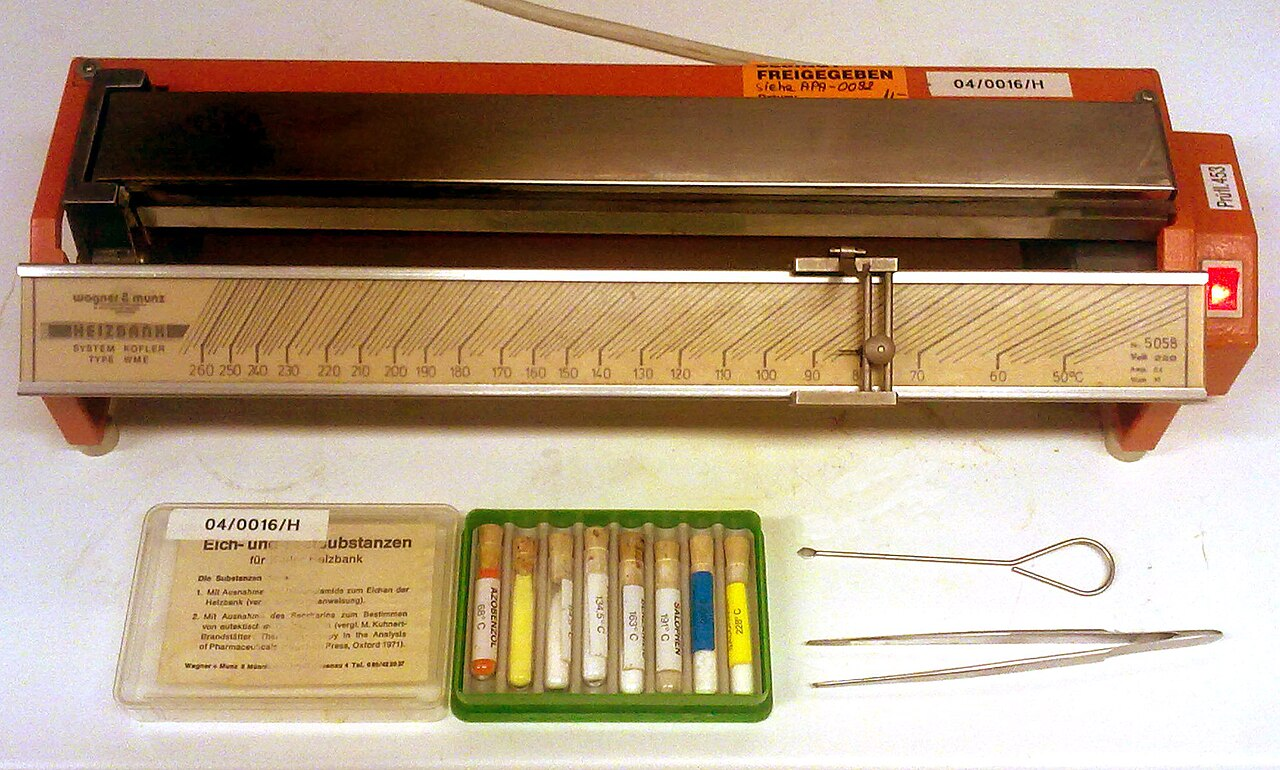
\includegraphics[width=0.62\linewidth]{images/book2/kofler-bench.jpg}

{\small Un banco calefactor (banco Kofler): una banda metálica calentada
por un extremo, con un gradiente de temperatura a lo largo de ella; el
sólido, espolvoreado sobre la banda, funde más allá de una línea nítida,
que se lee en la escala con el cursor. La caja contiene sustancias de
referencia de punto de fusión conocido, que sirven para calibrarlo.
Foto: HBR, CC BY-SA 3.0, Wikimedia Commons.}
\end{omfigure}

\begin{method}[Medir un punto de fusión en un banco calefactor]\label{met:b1:lab-techniques-1:melting-point}
\begin{enumerate}
  \item Se enciende el banco con suficiente antelación: el gradiente
        tarda en estabilizarse.
  \item Se calibra con una sustancia de referencia pura que funda cerca
        del valor esperado, espolvoreada sobre la banda; se ajusta el
        cursor de modo que la escala marque su punto de fusión sobre la
        línea.
  \item Se espolvorean unos \omterm{def:b1:crystals-metals:crystal}{cristales} de la muestra seca desde el extremo
        frío hacia el caliente; se empujan adelante y atrás con la
        espátula y se coloca el cursor en el límite a partir del cual el
        sólido funde al instante.
  \item Se lee, se repite, se limpia la banda; se toma la media de las
        lecturas y se expresa la incertidumbre
        (\cref{met:b1:lab-techniques-1:report-result}).
\end{enumerate}
\end{method}

Una sustancia cristalina pura funde de forma nítida en su punto de
fusión; una impura empieza a fundir más abajo y funde a lo largo de un
intervalo de temperaturas, porque la impureza rebaja la temperatura a la
que coexisten el sólido y el líquido (la razón, el potencial químico de
un disolvente rebajado por un soluto, está en el volumen del segundo
año). Un punto de fusión muy por debajo del valor tabulado, o un
intervalo de fusión amplio, revelan por tanto impurezas; un valor
compatible con el tabulado, en el sentido de la \omterm{def:b1:lab-techniques-1:z-score}{desviación normalizada},
apoya la pureza sin demostrarla.

\begin{inthelab}[Calibrar el banco]
Las referencias se eligen de modo que enmarquen el valor esperado. La
acetanilida, que funde a \qty{114.3}{\celsius}, y el ácido benzoico, a
\qty{122.4}{\celsius}, son patrones clásicos para productos que funden
entre \qty{110}{\celsius} y \qty{130}{\celsius}; para la aspirina, un
patrón cercano a \qty{135}{\celsius} es todavía mejor. La propia aspirina
se descompone al fundir, de modo que su punto de fusión observado depende
de la rapidez del calentamiento: las tablas dan \qty{135}{\celsius} para
un calentamiento rápido, que es lo que hace un banco.
% ledger: mp:acetanilide, mp:benzoic, mp:aspirin
\end{inthelab}

Un líquido se identifica, y se comprueba su pureza, por su \emph{índice
de refracción} $n_D$, la razón entre la velocidad de la luz en el vacío y
su velocidad en el líquido, medida con la línea D amarilla del sodio a
una temperatura indicada (normalmente \qty{20}{\celsius}), con cuatro
decimales. El agua tiene $n_D = 1.333$; el etanol, 1.3611, y el
ciclohexano, 1.4266, a \qty{20}{\celsius}. El índice disminuye
ligeramente al aumentar la temperatura, por lo que el instrumento está
termostatizado.
% ledger: nD:water, nD:ethanol, nD:cyclohexane

\begin{omfigure}
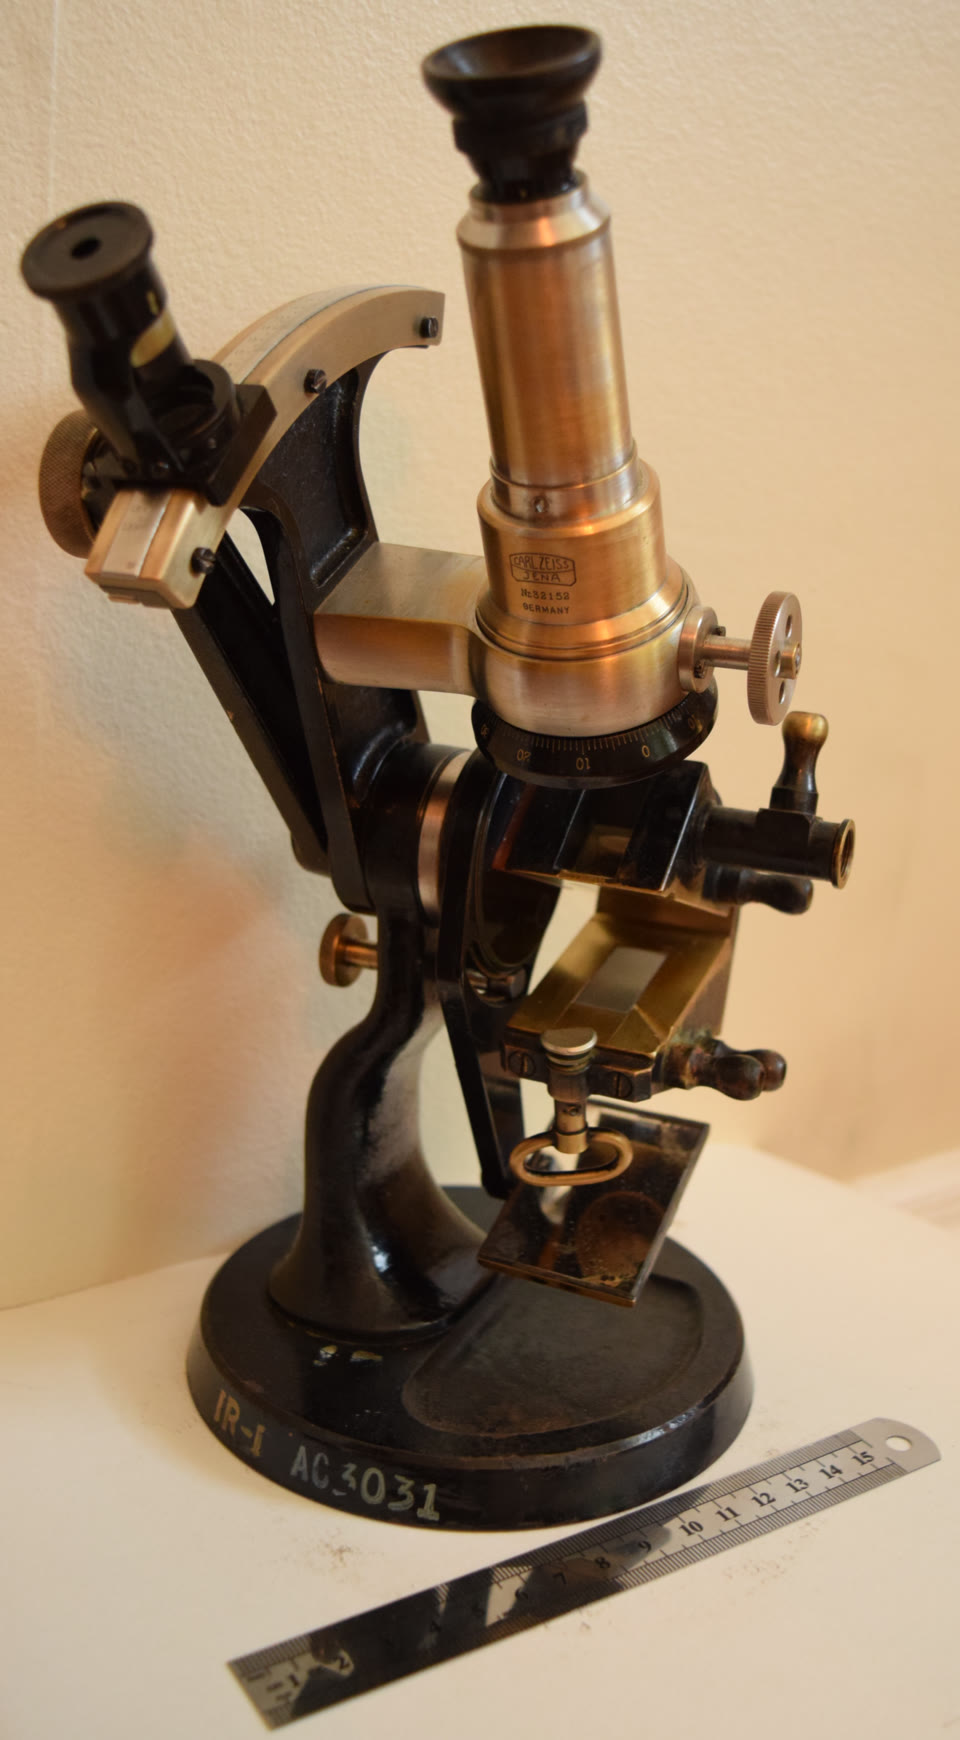
\includegraphics[height=6cm]{images/book2/abbe-refractometer.jpg}

{\small Un refractómetro de Abbe: una gota de líquido se extiende entre
dos prismas; el ocular muestra un campo mitad claro y mitad oscuro, y la
frontera, ajustada sobre la retícula, da el índice de refracción en la
escala. Foto: Foreade, CC BY-SA 4.0, Wikimedia Commons.}
\end{omfigure}

\section{Ejercicios}

\begin{exercise}[$\star$]\label{exo:b1:lab-techniques-1:1}
Una botella de propanona lleva los pictogramas GHS02 y GHS07 y las
indicaciones H225, H319 y H336. ¿Qué \omterm{def:b1:lab-techniques-1:ghs}{palabra de advertencia} lleva? ¿Qué
indicaciones describen un \omterm{def:b1:lab-techniques-1:hazard}{peligro} físico, y cuáles un peligro para la
salud? Nómbrense dos precauciones que exigen.
\end{exercise}

\begin{exercise}[$\star$]\label{exo:b1:lab-techniques-1:2}
¿\omterm{def:b1:lab-techniques-1:hazard}{Peligro} o \omterm{def:b1:lab-techniques-1:hazard}{riesgo}? (a) El ácido sulfúrico concentrado provoca
quemaduras graves. (b) Pesar \qty{50}{mg} de un polvo tóxico en una
vitrina de gases y con guantes expone poco al operador. (c) El sodio
libera hidrógeno con el agua. (d) El mismo disolvente es más peligroso
usado en caliente en un vaso abierto que en frío en una botella cerrada.
\end{exercise}

\begin{exercise}[$\star$]\label{exo:b1:lab-techniques-1:3}
En una placa de CCF, el frente del eluyente está \qty{6.0}{cm} por
encima de la línea de base; la muestra da manchas a \qty{2.1}{cm} y a
\qty{4.2}{cm}. Calcúlense sus $R_f$. Una referencia depositada en la
misma placa sube hasta \qty{4.2}{cm}: ¿qué puede concluirse y qué no?
\end{exercise}

\begin{exercise}[$\star$]\label{exo:b1:lab-techniques-1:4}
Una bureta graduada cada \qty{0.1}{mL} se lee a media división.
Calcúlese la \omterm{def:b1:lab-techniques-1:uncertainty}{incertidumbre típica} de una lectura y, después, la de un
volumen vertido, diferencia de dos lecturas.
\end{exercise}

\begin{exercise}[$\star\star$]\label{exo:b1:lab-techniques-1:5}
Cinco pesadas de la misma muestra dan \qty{0.2512}{g}, \qty{0.2508}{g},
\qty{0.2515}{g}, \qty{0.2510}{g} y \qty{0.2505}{g}. Calcúlense la media,
la desviación típica experimental y la \omterm{def:b1:lab-techniques-1:uncertainty}{incertidumbre típica} de la media,
y exprésese el resultado con $k = 2$.
\end{exercise}

\begin{exercise}[$\star\star$]\label{exo:b1:lab-techniques-1:6}
Un soluto de \omterm{def:b1:lab-techniques-1:partition-coefficient}{coeficiente de reparto} $K = 3$ entre un disolvente orgánico
y el agua se extrae de \qty{50}{mL} de agua con \qty{30}{mL} de
disolvente en total. Calcúlese la fracción extraída en una sola porción,
en dos porciones de \qty{15}{mL} y en tres de \qty{10}{mL}.
\end{exercise}

\begin{exercise}[$\star\star$]\label{exo:b1:lab-techniques-1:7}
Una \omterm{def:b1:titration-methods:titration}{valoración} da una concentración de \qty{0.1012}{mol/L} con una
\omterm{def:b1:lab-techniques-1:uncertainty}{incertidumbre típica} de \qty{0.0006}{mol/L}; la disolución se preparó a
\qty{0.1000}{mol/L} con una \omterm{def:b1:lab-techniques-1:uncertainty}{incertidumbre típica} de \qty{0.0002}{mol/L}.
¿Son compatibles los dos valores? ¿Y si la incertidumbre de la \omterm{def:b1:titration-methods:titration}{valoración}
hubiera sido de \qty{0.0004}{mol/L}?
\end{exercise}

\begin{exercise}[$\star\star$]\label{exo:b1:lab-techniques-1:8}
Las \omterm{def:b1:precipitation:solubility}{solubilidades} (valores ilustrativos, \unit{g} por \qty{100}{mL}) de un
sólido en tres disolventes son: disolvente P, 1.5 en frío y 2.0 en
ebullición; disolvente Q, 0.3 en frío y 12 en ebullición; disolvente R, 9
en frío y 25 en ebullición. ¿Qué disolvente conviene para una
\omterm{def:b1:lab-techniques-1:recrystallisation}{recristalización}, y por qué no los otros dos? Con el disolvente
adecuado, ¿cuál es la mayor fracción de \qty{5.0}{g} del sólido que puede
recuperarse, si se usa el mínimo de disolvente en ebullición y se enfría
la mezcla?
\end{exercise}

\begin{exercise}[$\star\star$]\label{exo:b1:lab-techniques-1:9}
Un líquido incoloro, termostatizado a \qty{20}{\celsius}, tiene
$n_D = 1.3612$. ¿Cuál de estos puede ser: agua, etanol o ciclohexano? ¿Por
qué se indica la temperatura? ¿Qué sugeriría un valor de 1.350?
\end{exercise}

\begin{exercise}[$\star\star\star$]\label{exo:b1:lab-techniques-1:10}
Con los datos del \cref{exo:b1:lab-techniques-1:6}, demuéstrese que, por
finamente que se divida el disolvente de \qty{30}{mL}, puede extraerse
como mucho una fracción $1 - \mathrm{e}^{-KV/V_a}$ del soluto, y
calcúlese. ¿Cuántas porciones alcanzan el \qty{99}{\percent} de ese
límite?
\end{exercise}

\begin{exercise}[$\star\star\star$]\label{exo:b1:lab-techniques-1:11}
Se sabe que una magnitud está entre $x_0 - a$ y $x_0 + a$, siendo más
probables los valores cercanos a $x_0$: su densidad es triangular,
$(a - |x - x_0|)/a^2$. Compruébese que está normalizada y demuéstrese que
su \omterm{def:b1:lab-techniques-1:uncertainty}{incertidumbre típica} es $a/\sqrt6$. Compárese con el caso
rectangular.
\end{exercise}

\begin{exercise}[$\star\star\star$]\label{exo:b1:lab-techniques-1:12}
Se prepara una disolución patrón disolviendo la muestra del
\cref{exo:b1:lab-techniques-1:5} (masa molar \qty{204.2}{g/mol}, de
incertidumbre despreciable) en un matraz aforado de \qty{100.00}{mL} cuyo
volumen tiene una \omterm{def:b1:lab-techniques-1:uncertainty}{incertidumbre típica} de \qty{0.06}{mL}. Calcúlense la
concentración y sus \omterm{def:b1:lab-techniques-1:uncertainty}{incertidumbres relativa} y expandida. ¿Qué fuente
domina?
\end{exercise}

\section{Problema: purificar la aspirina}

\begin{problem}[{Problema de fin de semana --- los peligros de una
síntesis, la recristalización de la aspirina bruta y su rendimiento, un
punto de fusión con sus incertidumbres de tipo A y de tipo B, y la
desviación normalizada respecto del valor tabulado}]
\label{pb:b1:lab-techniques-1:1}
Un estudiante prepara aspirina calentando \qty{2.00}{g} de ácido
salicílico con un exceso de anhídrido etanoico, y después recristaliza el
producto bruto. Masas molares (\unit{g/mol}): ácido salicílico
\ce{C7H6O3} 138.0, aspirina \ce{C9H8O4} 180.0, anhídrido etanoico
\ce{C4H6O3} 102.0. Etiquetas: ácido salicílico GHS05, GHS07, H302, H318;
anhídrido etanoico GHS02, GHS05, GHS06, GHS07, H226, H302, H314, H332;
aspirina GHS07, H302. \omterm{def:b1:precipitation:solubility}{Solubilidad} de la aspirina en agua:
\qty{3.3}{g/L} a \qty{25}{\celsius}. Punto de fusión tabulado de la
aspirina (calentamiento rápido): \qty{135}{\celsius}.
% ledger: ghs:salicylic, ghs:acetic-anhydride, ghs:aspirin, sol:aspirin-25,
% mp:aspirin, hstat:H318, hstat:H226, hstat:H314, hstat:H302

\medskip
\noindent\textbf{Parte I --- Los \omterm{def:b1:lab-techniques-1:hazard}{peligros}.}
\begin{enumerate}
  \item ¿Qué significa cada pictograma de la etiqueta del anhídrido
        etanoico?
  \item ¿Qué \omterm{def:b1:lab-techniques-1:ghs}{palabra de advertencia} lleva la etiqueta del ácido
        salicílico? ¿Y la de la aspirina?
  \item El anhídrido etanoico tiene los \omterm{def:b1:lab-techniques-1:hazard}{peligros} más graves. Explíquese
        cómo puede hacerse pequeño, sin embargo, el \omterm{def:b1:lab-techniques-1:hazard}{riesgo} de manipular
        \qty{5}{mL} de él.
  \item ¿Qué indicaciones del anhídrido exigen gafas y guantes, y cuáles
        la vitrina de gases y la ausencia de llamas?
  \item ¿Qué se hace de inmediato si una gota de anhídrido llega a un ojo?
  \item El filtrado de la \omterm{def:b1:lab-techniques-1:recrystallisation}{recristalización} contiene ácido etanoico y un
        poco de etanol en agua. ¿Adónde va?
\end{enumerate}

\noindent\textbf{Parte II --- Síntesis y \omterm{def:b1:lab-techniques-1:recrystallisation}{recristalización}.}
\begin{enumerate}[resume]
  \item Escríbase la ecuación de la síntesis, con el ácido etanoico
        \ce{C2H4O2} como subproducto, y compruébese que está ajustada.
  \item Calcúlense la cantidad de ácido salicílico y la masa máxima de
        aspirina.
  \item El producto bruto seco pesa \qty{2.41}{g}. ¿Por qué no puede
        omitirse la \omterm{def:b1:lab-techniques-1:recrystallisation}{recristalización}, aunque esto sea el
        \qty{92}{\percent} del máximo?
  \item La aspirina se recristaliza en un poco de etanol completado con
        agua caliente. ¿Por qué la propiedad que importa es la \omterm{def:b1:precipitation:solubility}{solubilidad}
        en agua a \qty{25}{\celsius}, comparada con la \omterm{def:b1:precipitation:solubility}{solubilidad} cerca de
        la ebullición?
  \item ¿Por qué se disuelve el sólido bruto en el mínimo de disolvente
        caliente?
  \item ¿Por qué se enfría la disolución lentamente y después en hielo?
  \item Salen del embudo \qty{40}{mL} de filtrado a \qty{25}{\celsius} y,
        después, \qty{5}{mL} de agua de lavado. Estímese la masa de
        aspirina que se pierde con ellos.
  \item El producto puro y seco pesa \qty{1.95}{g}. Calcúlese el
        \omterm{def:b1:extent-q-and-k:fractional-extent}{rendimiento}.
\end{enumerate}

\noindent\textbf{Parte III --- El punto de fusión.}
\begin{enumerate}[resume]
  \item Seis lecturas en el banco, calibrado justo antes, dan 134, 135,
        133, 135, 134 y \qty{136}{\celsius}. Calcúlese la media.
  \item Calcúlese la desviación típica experimental.
  \item Dedúzcase la \omterm{def:b1:lab-techniques-1:uncertainty}{incertidumbre típica} de tipo A de la media.
  \item Cada lectura se hace al grado más próximo. Calcúlese la
        incertidumbre de lectura de tipo B.
  \item La calibración del banco está garantizada a
        $\pm\qty{1}{\celsius}$. Calcúlense la incertidumbre de tipo B
        correspondiente y, después, la \omterm{def:b1:lab-techniques-1:uncertainty}{incertidumbre típica} combinada.
  \item Exprésese el punto de fusión con su \omterm{def:b1:lab-techniques-1:uncertainty}{incertidumbre expandida}
        ($k = 2$).
  \item El producto bruto de un compañero funde entre 120 y
        \qty{128}{\celsius}. ¿Qué indica esto?
\end{enumerate}

\noindent\textbf{Parte IV --- Comparación con la referencia.}
\begin{enumerate}[resume]
  \item El valor tabulado se da a la unidad. ¿Qué \omterm{def:b1:lab-techniques-1:uncertainty}{incertidumbre típica}
        implica?
  \item En una placa de CCF (frente a \qty{6.0}{cm}), el producto bruto
        muestra manchas a \qty{2.3}{cm} y a \qty{3.3}{cm}; el ácido
        salicílico, una mancha a \qty{2.3}{cm}; el producto recristalizado,
        una mancha a \qty{3.3}{cm}. Calcúlense los valores de $R_f$ y
        conclúyase.
  \item ¿Por qué depende el punto de fusión de la aspirina de la
        velocidad de calentamiento?
  \item Calcúlese la \omterm{def:b1:lab-techniques-1:z-score}{desviación normalizada} $z$ entre los puntos de fusión
        medido y tabulado, y dígase si son compatibles.
\end{enumerate}
\end{problem}
